\def\angle{0}
\def\radius{3}

% Quick pack breakdown Annapurna 2017
% pack      1185   13,72
% photo	    1400   16,21
% sleeping  1530   17,72
% clothing  3230   37,41
% safety    1040   12,05
% walking   249    2,88
% total     8634   100,00

\begin{figure}[H]
\centering

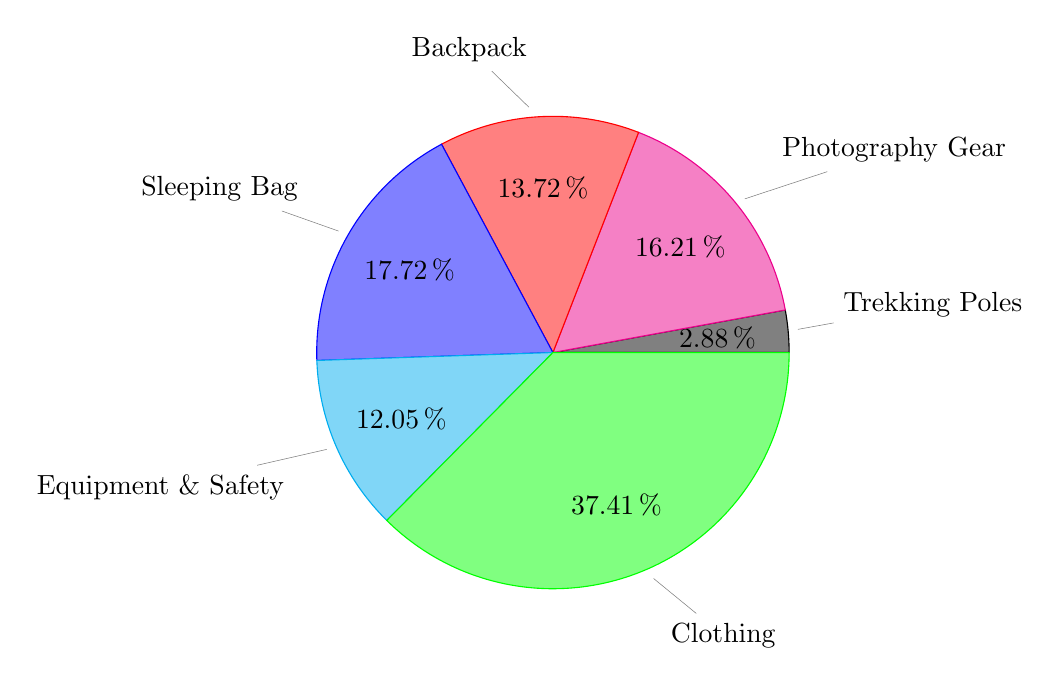
\begin{tikzpicture}
  \foreach \percent/\name/\color in {
      2.88/Trekking Poles/black,
      16.21/Photography Gear/magenta,
      13.72/Backpack/red,
      17.72/Sleeping Bag/blue,
      12.05/Equipment \& Safety/cyan,
      37.41/Clothing/green,
    } {
      \ifx\percent\empty\else % If \percent is empty, do nothing
        \draw[fill={\color!50},draw={\color}] (0,0) -- (\angle:\radius)
          arc (\angle:\angle+\percent*3.6:\radius) -- cycle;
        \node at (\angle+0.5*\percent*3.6:0.7*\radius) {\percent\,\%};
        \node[pin=\angle+0.5*\percent*3.6:\name]
          at (\angle+0.5*\percent*3.6:\radius) {};
        \pgfmathparse{\angle+\percent*3.6}
        \xdef\angle{\pgfmathresult}
      \fi
    };
\end{tikzpicture}

\caption[Example of conventional base weight distribution]{Example of conventional base weight distribution for a 3 weeks backpacking trip with freezing temperatures, but no need for shelter}

\end{figure}
